\documentclass[11pt,a4paper]{article}
\usepackage{times}
\usepackage[margin=2cm]{geometry}
\usepackage{graphicx}
\usepackage{hyperref}

\title{In-Depth Grant Proposal: Investigating the Interplay Between Gut Microbiota and Brain-Gut Axis in Irritable Bowel Syndrome}
\author{Dr. Alex Johnson, Department of Gastroenterology, University of Bergen}
\date{November 27, 2023}

\begin{document}

\maketitle

\section{Introduction}
\subsection{Background}
Irritable Bowel Syndrome (IBS) is a prevalent gastrointestinal disorder affecting a significant portion of the global population. Recent studies suggest a critical role of gut microbiota and the brain-gut axis in the pathophysiology of IBS. Understanding this interplay is essential for developing more effective treatments and management strategies for IBS patients.

\subsection{Rationale}
Current treatments for IBS are often inadequate, addressing only the symptoms rather than the underlying causes. This study aims to elucidate the complex interactions between gut microbiota and the brain-gut axis, potentially uncovering new therapeutic targets.

\section{Objectives and Hypotheses}
The primary objective is to identify specific microbiota changes in IBS patients and understand how these changes influence brain-gut interactions and symptom severity. We hypothesize that certain microbiota profiles are strongly correlated with the severity of IBS symptoms and brain-gut axis activity.

\section{Study Design}
\subsection{Participants}
We will recruit 200 adult participants, 100 diagnosed with IBS and 100 healthy controls, ensuring a representative sample in terms of age, gender, and ethnicity.

\subsection{Methodology}
The methodology includes comprehensive microbiota profiling through stool samples, functional MRI scans to study brain-gut interactions, and regular psychological assessments over 18 months.

\subsection{Data Analysis}
Data will be analyzed using mixed models to examine the relationships between microbiota composition, brain-gut interactions, and symptom severity.

\section{Ethical Considerations}
This study will adhere to ethical standards, ensuring informed consent, data protection, and confidentiality. All procedures have been designed to minimize participant discomfort and risk.

\section{Expected Outcomes and Impact}
We anticipate significant findings that will enhance the understanding of IBS, potentially leading to the development of novel diagnostic and therapeutic approaches.

\section{Budget}
The total budget is estimated at 7,500,000 NOK, covering personnel, lab analysis, equipment, participant compensation, and other operational costs.

\section{Project Timeline and Milestones}
\begin{figure}[h]
\centering
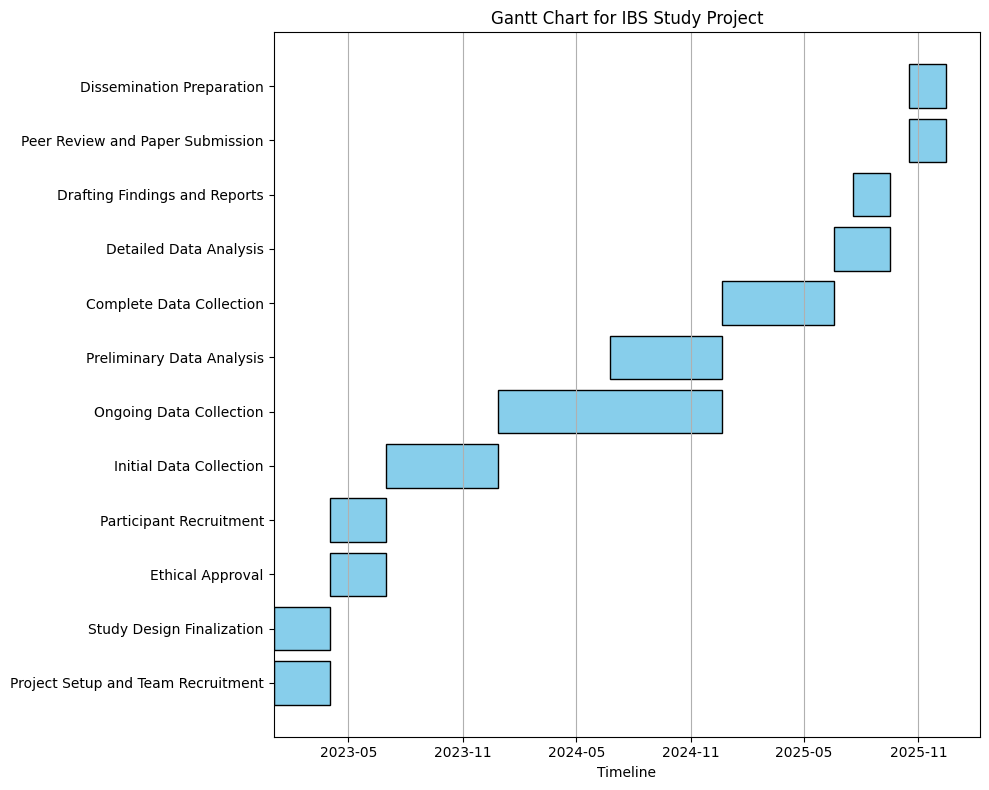
\includegraphics[width=0.9\textwidth]{./assets/gantt-chart-ibs.png}
\caption{Gantt Chart of the Project Timeline}
\end{figure}

\section{Conclusion}
This research promises to make substantial contributions to IBS research, with potential global impact on patient care and treatment strategies.

\begin{thebibliography}{9}
\bibitem{Tang2023}
Tang, Heyong et al. “Targeting the gut-microbiota-brain axis in irritable bowel disease to improve cognitive function - recent knowledge and emerging therapeutic opportunities.” \emph{Review Neuroscience}, vol. 34, no. 7, 2023, pp. 763-773. \href{https://doi.org/10.1515/revneuro-2022-0155}{DOI: 10.1515/revneuro-2022-0155}

\bibitem{Yuan2023}
Yuan, Yi et al. “Low-level inflammation, immunity, and brain-gut axis in IBS: unraveling the complex relationships.” \emph{Gut Microbes}, vol. 15, no. 2, 2023. \href{https://doi.org/10.1080/19490976.2023.2263209}{DOI: 10.1080/19490976.2023.2263209}

\bibitem{Mulder2023}
Mulder, Danique et al. “A systematic review exploring the association between the human gut microbiota and brain connectivity in health and disease.” \emph{Molecular Psychiatry}, 2023. \href{https://doi.org/10.1038/s41380-023-01972-w}{DOI: 10.1038/s41380-023-01972-w}

\bibitem{Mayer2023}
Mayer, Emeran A. et al. “The neurobiology of irritable bowel syndrome.” \emph{Molecular Psychiatry}, vol. 28, 2023, pp. 1451–1465. \href{https://doi.org/10.1038/s41380-023-01972-w}{DOI: 10.1038/s41380-023-01972-w}
\end{thebibliography}

\end{document}



